\documentclass[8pt,aspectratio=169]{beamer}
\usepackage[utf8]{inputenc}
\usepackage{graphicx}
\usepackage{amsmath,amssymb}
\usepackage{algorithm2e}
\usepackage{listings}
\usepackage{xcolor}
\usepackage{tikz}
\usepackage{pgfplots}
\pgfplotsset{compat=1.17}
\usepackage{subfigure}
\usepackage{hyperref}
\usepackage{tcolorbox}

% Theme settings
\usetheme{Frankfurt}
\usecolortheme{seahorse}
\setbeamertemplate{navigation symbols}{}
\setbeamertemplate{footline}[frame number]
\setbeamertemplate{section in toc}[sections numbered]
\setbeamertemplate{subsection in toc}[subsections numbered]

% Custom colors
\definecolor{darkblue}{RGB}{0,51,102}
\definecolor{lightblue}{RGB}{173,216,230}
\definecolor{codegreen}{RGB}{0,128,0}
\definecolor{codegray}{RGB}{150,150,150}
\definecolor{codepurple}{RGB}{128,0,128}
\definecolor{backcolor}{RGB}{245,245,245}

% Code listing settings
\lstset{
    backgroundcolor=\color{backcolor},
    basicstyle=\ttfamily\tiny,
    breakatwhitespace=false,
    breaklines=true,
    captionpos=b,
    commentstyle=\color{codegreen},
    keywordstyle=\color{blue},
    numberstyle=\tiny\color{codegray},
    stringstyle=\color{codepurple},
    showstringspaces=false,
    frame=single,
    numbers=left,
    language=Python
}

% Custom commands
\newcommand{\highlight}[1]{\textcolor{blue}{\textbf{#1}}}
\newcommand{\eqbox}[1]{\begin{tcolorbox}[colback=blue!5!white,colframe=blue!75!black]#1\end{tcolorbox}}
\newcommand{\given}{\mid}
\newcommand{\prob}[1]{P(#1)}
\DeclareMathOperator*{\argmax}{arg\,max}
\DeclareMathOperator*{\softmax}{softmax}

\title[Week 4: Seq2Seq]{Natural Language Processing}
\subtitle{Week 4: Sequence-to-Sequence Models}
\institute{Breaking the Fixed-Length Barrier}
\author{}
\date{}

\begin{document}

% Title slide
\begin{frame}
    \titlepage
\end{frame}

% Table of Contents
\begin{frame}{Week 4 Overview}
    \tableofcontents
\end{frame}

%=====================================
% PART 1: THE VARIABLE-LENGTH CHALLENGE
%=====================================

\section{Part 1: The Variable-Length Challenge}

\begin{frame}[t]{The Translation Revolution}
    \textbf{A Brief History:}
    
    \begin{itemize}
        \item \textbf{1950s-1990s}: Rule-based translation
        \begin{itemize}
            \item Dictionary lookups + grammar rules
            \item "The spirit is willing but the flesh is weak"
            \item $\rightarrow$ Russian $\rightarrow$ English: "The vodka is good but the meat is rotten"
        \end{itemize}
        
        \item \textbf{1990s-2010s}: Statistical machine translation
        \begin{itemize}
            \item Phrase-based models
            \item Required parallel corpora
        \end{itemize}
        
        \item \textbf{2014}: \highlight{Sequence-to-Sequence revolution}
        \begin{itemize}
            \item Neural networks learn to translate
            \item No rules, just examples!
        \end{itemize}
        
        \item \textbf{2017-now}: Attention and Transformers
        \begin{itemize}
            \item Near-human quality
            \item Powers Google Translate, DeepL
        \end{itemize}
    \end{itemize}
\end{frame}

\begin{frame}[t]{The Fundamental Problem}
    \textbf{Different languages = Different lengths!}
    
    \vspace{1em}
    \begin{center}
    \begin{tabular}{|l|l|c|}
        \hline
        \textbf{English} & \textbf{Translation} & \textbf{Words} \\
        \hline
        I love you & Je t'aime (French) & 3 $\rightarrow$ 2 \\
        I love you & Ich liebe dich (German) & 3 $\rightarrow$ 3 \\
        I love you & Aishiteru (Japanese) & 3 $\rightarrow$ 1 \\
        I love you & Eu te amo (Portuguese) & 3 $\rightarrow$ 3 \\
        \hline
    \end{tabular}
    \end{center}
    
    \vspace{1em}
    \textbf{The challenge:}
    \begin{itemize}
        \item Input length $\neq$ Output length
        \item Word order changes between languages
        \item One word can become many (and vice versa)
    \end{itemize}
    
    \vspace{1em}
    \colorbox{red!20}{
        \parbox{0.9\textwidth}{
            \centering
            RNNs produce one output per input - this won't work!
        }
    }
\end{frame}

\begin{frame}[t]{Where Fixed-Length Models Fail}
    \textbf{Naive Approach 1: Padding}
    \begin{itemize}
        \item Pad all sequences to maximum length
        \item Problem: Wastes computation, learns to ignore padding
    \end{itemize}
    
    \vspace{0.5em}
    \textbf{Naive Approach 2: Truncation}
    \begin{itemize}
        \item Cut sequences to fixed length
        \item Problem: Loses critical information!
    \end{itemize}
    
    \vspace{0.5em}
    \textbf{Naive Approach 3: Sliding Windows}
    \begin{itemize}
        \item Process in fixed-size chunks
        \item Problem: Breaks semantic units
    \end{itemize}
    
    \vspace{1em}
    \begin{center}
    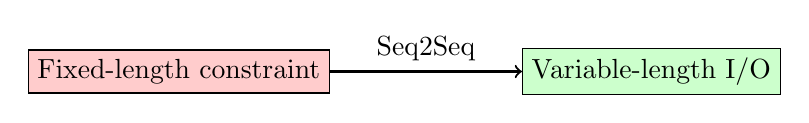
\begin{tikzpicture}
        \node[draw, rectangle, fill=red!20] (problem) at (0,0) {Fixed-length constraint};
        \node[draw, rectangle, fill=green!20] (solution) at (6,0) {Variable-length I/O};
        \draw[->, thick] (problem) -- (solution) node[midway, above] {Seq2Seq};
    \end{tikzpicture}
    \end{center}
\end{frame}

\begin{frame}[t]{Real-World Variable-Length Tasks}
    \textbf{Where we need flexible input/output:}
    
    \begin{columns}
    \column{0.5\textwidth}
    \textbf{Translation}
    \begin{itemize}
        \item Any language pair
        \item Technical documents
        \item Real-time conversation
    \end{itemize}
    
    \textbf{Summarization}
    \begin{itemize}
        \item Article $\rightarrow$ headline
        \item Book $\rightarrow$ abstract
        \item Meeting $\rightarrow$ minutes
    \end{itemize}
    
    \column{0.5\textwidth}
    \textbf{Dialog Systems}
    \begin{itemize}
        \item Question $\rightarrow$ answer
        \item Chat $\rightarrow$ response
        \item Command $\rightarrow$ action
    \end{itemize}
    
    \textbf{Code Generation}
    \begin{itemize}
        \item Comment $\rightarrow$ code
        \item Spec $\rightarrow$ implementation
        \item Bug description $\rightarrow$ fix
    \end{itemize}
    \end{columns}
    
    \vspace{1em}
    \colorbox{blue!20}{
        \parbox{0.9\textwidth}{
            \centering
            All these tasks have variable-length inputs AND outputs!
        }
    }
\end{frame}

\begin{frame}[t]{The Key Insight: Two-Stage Processing}
    \textbf{How humans translate:}
    
    \begin{enumerate}
        \item \textbf{Read and understand} the entire source sentence
        \item \textbf{Generate} the translation based on understanding
    \end{enumerate}
    
    \vspace{1em}
    \textbf{The Seq2Seq insight:}
    
    \begin{center}
    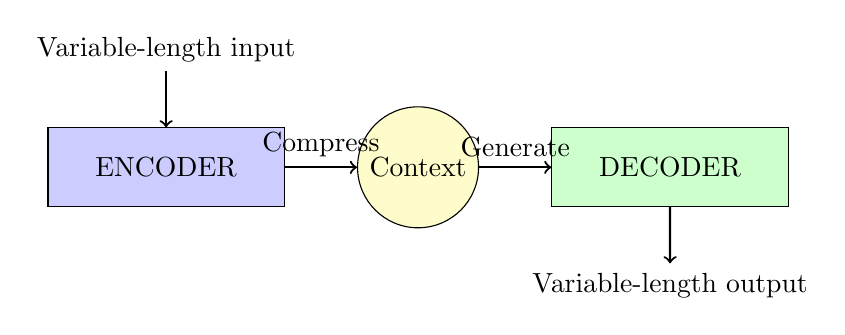
\begin{tikzpicture}[scale=0.8]
        % Encoder
        \node[draw, rectangle, fill=blue!20, minimum width=3cm, minimum height=1cm] 
            (encoder) at (0,0) {ENCODER};
        \node[above of=encoder, node distance=1.5cm] (input) {Variable-length input};
        \draw[->, thick] (input) -- (encoder);
        
        % Context
        \node[draw, circle, fill=yellow!20, minimum size=1.5cm] 
            (context) at (4,0) {Context};
        \draw[->, thick] (encoder) -- (context) node[midway, above] {Compress};
        
        % Decoder
        \node[draw, rectangle, fill=green!20, minimum width=3cm, minimum height=1cm] 
            (decoder) at (8,0) {DECODER};
        \draw[->, thick] (context) -- (decoder) node[midway, above] {Generate};
        
        \node[below of=decoder, node distance=1.5cm] (output) {Variable-length output};
        \draw[->, thick] (decoder) -- (output);
    \end{tikzpicture}
    \end{center}
    
    \vspace{1em}
    \highlight{Key: Fixed-size context vector bridges variable-length sequences!}
\end{frame}

\begin{frame}[t]{Evolution: Predicting the Next Word}
    \textbf{How each approach handles "next word prediction":}
    
    \vspace{0.5em}
    \begin{tabular}{|l|l|l|l|}
        \hline
        \textbf{Method} & \textbf{Context} & \textbf{Method} & \textbf{Output} \\
        \hline
        N-gram & Fixed n words & Count & Single word \\
        RNN & All previous & Hidden state & Single word \\
        \highlight{Seq2Seq} & \highlight{Entire input} & \highlight{Encode-decode} & \highlight{Full sequence} \\
        \hline
    \end{tabular}
    
    \vspace{1em}
    \textbf{Example: "How are you?" $\rightarrow$ "Comment allez-vous?"}
    
    \begin{itemize}
        \item \textbf{N-gram}: Would need to see exact phrase before
        \item \textbf{RNN}: Produces "How" $\rightarrow$ "Comment", "are" $\rightarrow$ ?, stuck!
        \item \textbf{Seq2Seq}: Reads full input, generates full output
    \end{itemize}
    
    \vspace{1em}
    \colorbox{green!20}{
        \parbox{0.9\textwidth}{
            Seq2Seq doesn't just predict next word - it generates entire sequences!
        }
    }
\end{frame}

%=====================================
% PART 2: THE ENCODER-DECODER ARCHITECTURE
%=====================================

\section{Part 2: The Encoder-Decoder Architecture}

\begin{frame}[t]{The Encoder: Compressing Meaning}
    \textbf{What the encoder does:}
    
    Process input sequence $\rightarrow$ Create fixed-size representation
    
    \vspace{1em}
    \eqbox{
        $\begin{aligned}
        h_t^{enc} &= \text{LSTM}(x_t, h_{t-1}^{enc}) & \text{Process each word} \\
        c &= h_T^{enc} & \text{Final hidden state = context}
        \end{aligned}$
    }
    
    \vspace{1em}
    \textbf{Step-by-step example:} "I love NLP"
    
    \begin{center}
    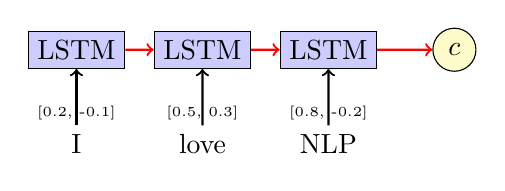
\begin{tikzpicture}[scale=0.8]
        % Input words
        \node at (0, 0) {I};
        \node at (2, 0) {love};
        \node at (4, 0) {NLP};
        
        % LSTM cells
        \node[draw, rectangle, fill=blue!20] (lstm1) at (0, 1.5) {LSTM};
        \node[draw, rectangle, fill=blue!20] (lstm2) at (2, 1.5) {LSTM};
        \node[draw, rectangle, fill=blue!20] (lstm3) at (4, 1.5) {LSTM};
        
        % Connections
        \draw[->, thick] (0, 0.3) -- (lstm1);
        \draw[->, thick] (2, 0.3) -- (lstm2);
        \draw[->, thick] (4, 0.3) -- (lstm3);
        
        \draw[->, thick, red] (lstm1) -- (lstm2);
        \draw[->, thick, red] (lstm2) -- (lstm3);
        
        % Context vector
        \node[draw, circle, fill=yellow!20] (context) at (6, 1.5) {$c$};
        \draw[->, thick, red] (lstm3) -- (context);
        
        % Hidden state values
        \node[below of=lstm1, node distance=0.8cm] {\tiny [0.2, -0.1]};
        \node[below of=lstm2, node distance=0.8cm] {\tiny [0.5, 0.3]};
        \node[below of=lstm3, node distance=0.8cm] {\tiny [0.8, -0.2]};
    \end{tikzpicture}
    \end{center}
    
    \highlight{Context vector $c$ captures the meaning of entire input!}
\end{frame}

\begin{frame}[t]{The Decoder: Generating from Context}
    \textbf{What the decoder does:}
    
    Use context vector $\rightarrow$ Generate output sequence
    
    \vspace{1em}
    \eqbox{
        $\begin{aligned}
        h_t^{dec} &= \text{LSTM}(y_{t-1}, h_{t-1}^{dec}, c) & \text{Generate each word} \\
        y_t &= \softmax(W \cdot h_t^{dec}) & \text{Predict next word}
        \end{aligned}$
    }
    
    \vspace{1em}
    \textbf{Generation process:} Context $\rightarrow$ "J'aime le NLP"
    
    \begin{center}
    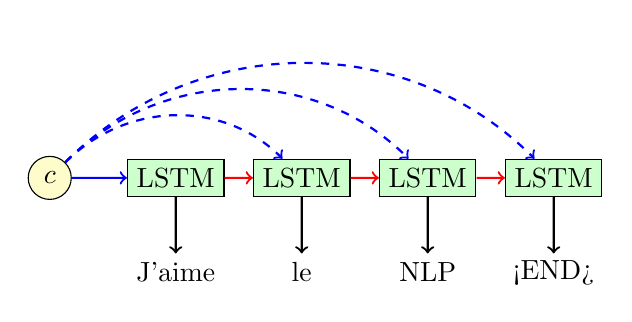
\begin{tikzpicture}[scale=0.8]
        % Context
        \node[draw, circle, fill=yellow!20] (context) at (0, 1.5) {$c$};
        
        % Decoder LSTMs
        \node[draw, rectangle, fill=green!20] (lstm1) at (2, 1.5) {LSTM};
        \node[draw, rectangle, fill=green!20] (lstm2) at (4, 1.5) {LSTM};
        \node[draw, rectangle, fill=green!20] (lstm3) at (6, 1.5) {LSTM};
        \node[draw, rectangle, fill=green!20] (lstm4) at (8, 1.5) {LSTM};
        
        % Connections from context
        \draw[->, thick, blue] (context) -- (lstm1);
        \draw[->, thick, blue, dashed] (context) to[out=45,in=135] (lstm2);
        \draw[->, thick, blue, dashed] (context) to[out=45,in=135] (lstm3);
        \draw[->, thick, blue, dashed] (context) to[out=45,in=135] (lstm4);
        
        % Sequential connections
        \draw[->, thick, red] (lstm1) -- (lstm2);
        \draw[->, thick, red] (lstm2) -- (lstm3);
        \draw[->, thick, red] (lstm3) -- (lstm4);
        
        % Output words
        \node at (2, 0) {J'aime};
        \node at (4, 0) {le};
        \node at (6, 0) {NLP};
        \node at (8, 0) {<END>};
        
        \draw[->, thick] (lstm1) -- (2, 0.3);
        \draw[->, thick] (lstm2) -- (4, 0.3);
        \draw[->, thick] (lstm3) -- (6, 0.3);
        \draw[->, thick] (lstm4) -- (8, 0.3);
    \end{tikzpicture}
    \end{center}
\end{frame}

\begin{frame}[fragile,t]{Complete Seq2Seq Implementation}
    \textbf{Minimal working seq2seq in 20 lines:}
    
    \begin{lstlisting}
class Seq2Seq:
    def __init__(self, vocab_size, hidden_size):
        self.encoder = LSTM(vocab_size, hidden_size)
        self.decoder = LSTM(vocab_size, hidden_size)
        self.output_proj = Linear(hidden_size, vocab_size)
    
    def encode(self, source_sequence):
        h = zeros(hidden_size)
        for word in source_sequence:
            h, _ = self.encoder(embed(word), h)
        return h  # This is our context vector
    
    def decode(self, context, max_length=50):
        h = context
        word = START_TOKEN
        output = []
        for _ in range(max_length):
            h, _ = self.decoder(embed(word), h)
            word = softmax(self.output_proj(h))
            output.append(word)
            if word == END_TOKEN: break
        return output
    \end{lstlisting}
\end{frame}

\begin{frame}[t]{Teacher Forcing: Training Trick}
    \textbf{Problem:} Early in training, decoder makes mistakes $\rightarrow$ compounds errors
    
    \vspace{1em}
    \textbf{Solution:} During training, feed correct previous word (not predicted)
    
    \begin{columns}
    \column{0.5\textwidth}
    \textbf{Without Teacher Forcing:}
    \begin{itemize}
        \item Target: "J'aime le NLP"
        \item Predicts: "Je"
        \item Next input: "Je" (wrong!)
        \item Predicts: "suis" (more wrong!)
        \item Cascade of errors...
    \end{itemize}
    
    \column{0.5\textwidth}
    \textbf{With Teacher Forcing:}
    \begin{itemize}
        \item Target: "J'aime le NLP"
        \item Predicts: "Je" (wrong)
        \item Next input: "J'aime" (correct!)
        \item Predicts: "le" (learning!)
        \item Faster convergence
    \end{itemize}
    \end{columns}
    
    \vspace{1em}
    \colorbox{yellow!20}{
        \parbox{0.9\textwidth}{
            At test time: Use predicted words (no teacher forcing)
        }
    }
\end{frame}

\begin{frame}[t]{Numerical Example: Translation Step-by-Step}
    \textbf{Translating:} "cat" $\rightarrow$ "chat"
    
    \vspace{0.5em}
    \textbf{Encoding:}
    \begin{itemize}
        \item Input embedding: "cat" $\rightarrow$ [0.3, -0.2, 0.8, 0.1]
        \item Encoder LSTM: [0.3, -0.2, 0.8, 0.1] $\rightarrow$ context [0.5, 0.1, -0.3, 0.7]
    \end{itemize}
    
    \vspace{0.5em}
    \textbf{Decoding:}
    \begin{enumerate}
        \item Start with context: [0.5, 0.1, -0.3, 0.7]
        \item Decoder LSTM step 1:
        \begin{itemize}
            \item Input: <START> + context
            \item Hidden: [0.4, 0.2, -0.1, 0.6]
            \item Output scores: \{chat: 2.3, chien: 0.8, maison: 0.2, ...\}
            \item Softmax: \{chat: 0.73, chien: 0.15, maison: 0.03, ...\}
            \item Select: "chat"
        \end{itemize}
        \item Decoder LSTM step 2:
        \begin{itemize}
            \item Input: "chat" + hidden
            \item Output: <END> token
        \end{itemize}
    \end{enumerate}
    
    \highlight{Result: "cat" successfully translated to "chat"!}
\end{frame}

\begin{frame}[t]{Bidirectional Encoders: Looking Both Ways}
    \textbf{Problem:} Forward LSTM only sees past context
    
    \vspace{0.5em}
    \textbf{Solution:} Process sequence in both directions!
    
    \begin{center}
    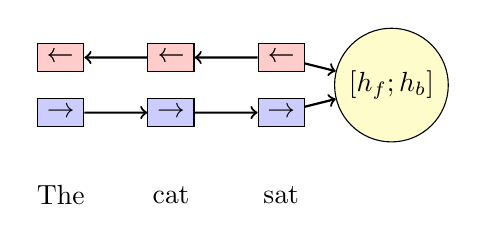
\begin{tikzpicture}[scale=0.7]
        % Input
        \node at (2, 0) {The};
        \node at (4, 0) {cat};
        \node at (6, 0) {sat};
        
        % Forward LSTM
        \node[draw, rectangle, fill=blue!20] (f1) at (2, 1.5) {$\rightarrow$};
        \node[draw, rectangle, fill=blue!20] (f2) at (4, 1.5) {$\rightarrow$};
        \node[draw, rectangle, fill=blue!20] (f3) at (6, 1.5) {$\rightarrow$};
        
        % Backward LSTM
        \node[draw, rectangle, fill=red!20] (b1) at (2, 2.5) {←};
        \node[draw, rectangle, fill=red!20] (b2) at (4, 2.5) {←};
        \node[draw, rectangle, fill=red!20] (b3) at (6, 2.5) {←};
        
        % Connections
        \draw[->, thick] (f1) -- (f2);
        \draw[->, thick] (f2) -- (f3);
        \draw[<-, thick] (b1) -- (b2);
        \draw[<-, thick] (b2) -- (b3);
        
        % Concatenation
        \node[draw, circle, fill=yellow!20] (concat) at (8, 2) {$[h_f; h_b]$};
        \draw[->, thick] (f3) -- (concat);
        \draw[->, thick] (b3) -- (concat);
    \end{tikzpicture}
    \end{center}
    
    \vspace{0.5em}
    \textbf{Benefits:}
    \begin{itemize}
        \item "cat" knows about "sat" (future context)
        \item Better representation of each word
        \item Standard in modern seq2seq
    \end{itemize}
\end{frame}

%=====================================
% PART 3: THE INFORMATION BOTTLENECK
%=====================================

\section{Part 3: The Information Bottleneck Problem}

\begin{frame}[t]{When Context Vectors Fail}
    \textbf{The bottleneck:} Compressing everything into fixed-size vector
    
    \vspace{1em}
    \begin{center}
    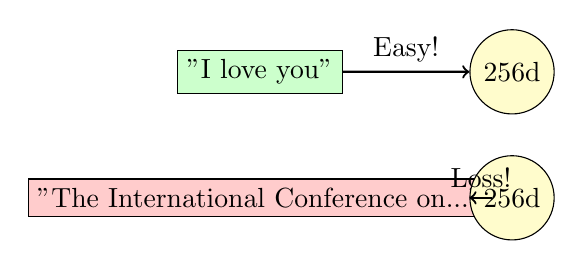
\begin{tikzpicture}[scale=0.8]
        % Short sentence
        \node[draw, rectangle, fill=green!20, minimum width=2cm] (short) at (0, 2) 
            {"I love you"};
        \node[draw, circle, fill=yellow!20] (context1) at (4, 2) {256d};
        \draw[->, thick] (short) -- (context1) node[midway, above] {Easy!};
        
        % Long sentence
        \node[draw, rectangle, fill=red!20, minimum width=5cm] (long) at (0, 0) 
            {"The International Conference on..."};
        \node[draw, circle, fill=yellow!20] (context2) at (4, 0) {256d};
        \draw[->, thick] (long) -- (context2) node[midway, above] {Loss!};
    \end{tikzpicture}
    \end{center}
    
    \vspace{1em}
    \textbf{Information theory perspective:}
    \begin{itemize}
        \item 256-dimensional vector = ~1KB of information
        \item Long document = ~100KB of information
        \item \highlight{Cannot compress 100KB $\rightarrow$ 1KB without loss!}
    \end{itemize}
\end{frame}

\begin{frame}[t]{Visualizing Information Loss}
    \textbf{Performance vs. Sentence Length:}
    
    \begin{center}
    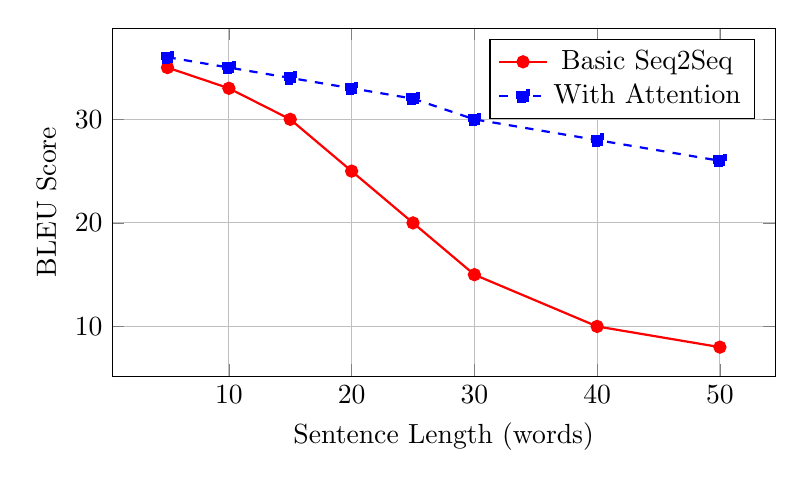
\begin{tikzpicture}
        \begin{axis}[
            xlabel={Sentence Length (words)},
            ylabel={BLEU Score},
            width=10cm,
            height=6cm,
            grid=major,
            legend pos=north east
        ]
        
        % Seq2Seq performance
        \addplot[color=red, thick, mark=*] coordinates {
            (5, 35) (10, 33) (15, 30) (20, 25) (25, 20) (30, 15) (40, 10) (50, 8)
        };
        \addlegendentry{Basic Seq2Seq}
        
        % With attention (preview)
        \addplot[color=blue, thick, mark=square*, dashed] coordinates {
            (5, 36) (10, 35) (15, 34) (20, 33) (25, 32) (30, 30) (40, 28) (50, 26)
        };
        \addlegendentry{With Attention}
        
        \end{axis}
    \end{tikzpicture}
    \end{center}
    
    \highlight{Performance degrades drastically after 15-20 words!}
\end{frame}

\begin{frame}[t]{Real Examples of Bottleneck Failures}
    \textbf{Legal Document Translation:}
    
    \begin{tcolorbox}[colback=red!5!white,colframe=red!75!black]
    \textbf{Input (50 words):} "The party of the first part hereby agrees to indemnify and hold harmless the party of the second part from any and all claims, damages, losses, and expenses, including but not limited to reasonable attorney's fees, arising from..."
    
    \textbf{Output:} "La partie accepte de payer." (The party agrees to pay.)
    
    \textbf{Lost:} Who indemnifies whom, what claims, legal details!
    \end{tcolorbox}
    
    \vspace{0.5em}
    \textbf{Technical Manual Translation:}
    
    \begin{tcolorbox}[colback=red!5!white,colframe=red!75!black]
    \textbf{Input (35 words):} "To replace the filter, first disconnect power, then remove the four screws on the top panel, lift carefully to avoid damaging the sensor wire, and locate the filter housing behind the main unit."
    
    \textbf{Output:} "Remplacer le filtre." (Replace the filter.)
    
    \textbf{Lost:} All safety steps and detailed instructions!
    \end{tcolorbox}
\end{frame}

\begin{frame}[t]{Why Fixed Context Fails: Memory Analogy}
    \textbf{Human memory analogy:}
    
    \vspace{0.5em}
    Imagine memorizing a book by reading it once and storing it in your mind as a single "feeling"
    
    \vspace{1em}
    \begin{columns}
    \column{0.5\textwidth}
    \textbf{Short story (5 pages):}
    \begin{itemize}
        \item Can remember plot
        \item Can recall characters
        \item Can retell accurately
    \end{itemize}
    
    \column{0.5\textwidth}
    \textbf{Novel (500 pages):}
    \begin{itemize}
        \item Forget early chapters
        \item Mix up characters
        \item Only remember gist
    \end{itemize}
    \end{columns}
    
    \vspace{1em}
    \colorbox{yellow!20}{
        \parbox{0.9\textwidth}{
            \centering
            Humans don't compress books into single thoughts - \\
            we refer back to specific parts when needed!
        }
    }
    
    \vspace{0.5em}
    \highlight{This insight leads to the attention mechanism...}
\end{frame}

%=====================================
% PART 4: ATTENTION MECHANISM
%=====================================

\section{Part 4: Attention Mechanism - The Game Changer}

\begin{frame}[t]{The Attention Revolution (Bahdanau et al., 2015)}
    \textbf{The key insight:} Don't compress everything - look back at what you need!
    
    \vspace{1em}
    \begin{center}
    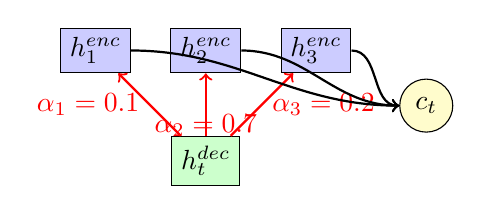
\begin{tikzpicture}[scale=0.7]
        % Encoder states
        \node[draw, rectangle, fill=blue!20] (e1) at (0, 2) {$h_1^{enc}$};
        \node[draw, rectangle, fill=blue!20] (e2) at (2, 2) {$h_2^{enc}$};
        \node[draw, rectangle, fill=blue!20] (e3) at (4, 2) {$h_3^{enc}$};
        
        % Decoder state
        \node[draw, rectangle, fill=green!20] (decoder) at (2, 0) {$h_t^{dec}$};
        
        % Attention weights
        \draw[->, thick, red] (decoder) -- (e1) node[midway, left] {$\alpha_1=0.1$};
        \draw[->, thick, red] (decoder) -- (e2) node[midway, below] {$\alpha_2=0.7$};
        \draw[->, thick, red] (decoder) -- (e3) node[midway, right] {$\alpha_3=0.2$};
        
        % Context vector
        \node[draw, circle, fill=yellow!20] (context) at (6, 1) {$c_t$};
        \draw[->, thick] (e1) to[out=0,in=180] (context);
        \draw[->, thick] (e2) to[out=0,in=180] (context);
        \draw[->, thick] (e3) to[out=0,in=180] (context);
    \end{tikzpicture}
    \end{center}
    
    \vspace{0.5em}
    \textbf{How attention works:}
    \begin{enumerate}
        \item Keep ALL encoder hidden states (not just last)
        \item At each decoder step, compute relevance scores
        \item Create weighted sum of encoder states
        \item Use this dynamic context for generation
    \end{enumerate}
\end{frame}

\begin{frame}[t]{Attention Mathematics Made Simple}
    \textbf{Three steps to attention:}
    
    \vspace{0.5em}
    \textbf{1. Score:} How relevant is each encoder state?
    \eqbox{
        $score(h_t^{dec}, h_i^{enc}) = h_t^{dec} \cdot h_i^{enc}$ \quad (dot product)
    }
    
    \textbf{2. Normalize:} Convert scores to probabilities
    \eqbox{
        $\alpha_i = \frac{\exp(score_i)}{\sum_j \exp(score_j)}$ \quad (softmax)
    }
    
    \textbf{3. Combine:} Weighted sum of encoder states
    \eqbox{
        $c_t = \sum_i \alpha_i \cdot h_i^{enc}$
    }
    
    \vspace{0.5em}
    \textbf{Intuition:} The decoder "asks" each encoder state: \\
    "How much should I pay attention to you right now?"
\end{frame}

\begin{frame}[t]{Attention in Action: Translation Example}
    \textbf{Translating:} "The cat sat" $\rightarrow$ "Le chat s'est assis"
    
    \vspace{0.5em}
    \begin{center}
    \begin{tabular}{|l|c|c|c|}
        \hline
        \textbf{Generating} & \multicolumn{3}{c|}{\textbf{Attention Weights}} \\
        \cline{2-4}
        & The & cat & sat \\
        \hline
        Le & \colorbox{green!30}{0.7} & 0.2 & 0.1 \\
        chat & 0.1 & \colorbox{green!30}{0.8} & 0.1 \\
        s'est & 0.1 & 0.1 & \colorbox{green!30}{0.8} \\
        assis & 0.1 & 0.2 & \colorbox{green!30}{0.7} \\
        \hline
    \end{tabular}
    \end{center}
    
    \vspace{0.5em}
    \textbf{Observations:}
    \begin{itemize}
        \item "Le" attends to "The" (articles align)
        \item "chat" attends to "cat" (nouns align)
        \item "s'est assis" attends to "sat" (verbs align)
        \item Model learns alignment without explicit rules!
    \end{itemize}
\end{frame}

\begin{frame}[fragile,t]{Implementing Attention}
    \begin{lstlisting}
def attention(decoder_hidden, encoder_outputs):
    """
    decoder_hidden: current decoder state [hidden_size]
    encoder_outputs: all encoder states [seq_len, hidden_size]
    """
    # Step 1: Calculate scores
    scores = torch.dot(decoder_hidden, encoder_outputs.T)
    # scores shape: [seq_len]
    
    # Step 2: Normalize with softmax
    attention_weights = torch.softmax(scores, dim=0)
    # attention_weights shape: [seq_len], sum to 1
    
    # Step 3: Weighted sum of encoder outputs
    context = torch.sum(
        attention_weights.unsqueeze(1) * encoder_outputs, 
        dim=0
    )
    # context shape: [hidden_size]
    
    return context, attention_weights

# Example usage:
# context, weights = attention(decoder_h, all_encoder_h)
# decoder_h_new = LSTM(input, decoder_h, context)
    \end{lstlisting}
\end{frame}

\begin{frame}[t]{Types of Attention}
    \textbf{Different ways to compute attention scores:}
    
    \vspace{0.5em}
    \begin{enumerate}
        \item \textbf{Dot Product (Luong):}
        \begin{itemize}
            \item $score = h_t^{dec} \cdot h_i^{enc}$
            \item Fast, no parameters
            \item Requires same dimensionality
        \end{itemize}
        
        \item \textbf{Additive (Bahdanau):}
        \begin{itemize}
            \item $score = v^T \tanh(W_1 h_t^{dec} + W_2 h_i^{enc})$
            \item More flexible
            \item Can handle different dimensions
        \end{itemize}
        
        \item \textbf{Multiplicative:}
        \begin{itemize}
            \item $score = h_t^{dec} W h_i^{enc}$
            \item Learnable weight matrix
            \item Balance of flexibility and speed
        \end{itemize}
    \end{enumerate}
    
    \vspace{0.5em}
    \colorbox{blue!20}{
        \parbox{0.9\textwidth}{
            All types learn to align source and target automatically!
        }
    }
\end{frame}

\begin{frame}[t]{Attention Visualization: What Model Sees}
    \textbf{Real attention heatmap from translation:}
    
    \begin{center}
    % \includegraphics[width=0.8\textwidth]{../figures/attention_heatmap.pdf}
    \textit{[Attention heatmap visualization will be generated]}
    \end{center}
    
    \textbf{Key insights:}
    \begin{itemize}
        \item Diagonal pattern = word alignment
        \item Off-diagonal = reordering between languages
        \item Brightness = attention strength
        \item Model learns linguistic structure!
    \end{itemize}
\end{frame}

\begin{frame}[t]{Performance Impact of Attention}
    \textbf{BLEU scores on WMT'14 English-French:}
    
    \vspace{0.5em}
    \begin{center}
    \begin{tabular}{|l|c|c|}
        \hline
        \textbf{Model} & \textbf{BLEU Score} & \textbf{Improvement} \\
        \hline
        Basic Seq2Seq & 25.3 & baseline \\
        + Bidirectional encoder & 27.1 & +1.8 \\
        + Attention & 31.7 & +6.4 \\
        + Beam search & 33.2 & +7.9 \\
        \hline
        Google Translate (2016) & 38.9 & +13.6 \\
        Transformer (2017) & 41.8 & +16.5 \\
        \hline
    \end{tabular}
    \end{center}
    
    \vspace{0.5em}
    \colorbox{green!20}{
        \parbox{0.9\textwidth}{
            \centering
            Attention gives 25\% relative improvement! \\
            This breakthrough enabled near-human translation quality.
        }
    }
\end{frame}

%=====================================
% SUMMARY
%=====================================

\begin{frame}[t]{Summary: Breaking the Fixed-Length Barrier}
    \textbf{What we learned:}
    
    \begin{enumerate}
        \item \textbf{Variable-length challenge:}
        \begin{itemize}
            \item Different languages have different lengths
            \item Fixed-size models fail
        \end{itemize}
        
        \item \textbf{Encoder-Decoder architecture:}
        \begin{itemize}
            \item Separate compression from generation
            \item Enables variable input/output
        \end{itemize}
        
        \item \textbf{Information bottleneck:}
        \begin{itemize}
            \item Fixed context loses information
            \item Performance degrades with length
        \end{itemize}
        
        \item \textbf{Attention mechanism:}
        \begin{itemize}
            \item Look back at all encoder states
            \item Dynamic, focused context
            \item Dramatic performance improvement
        \end{itemize}
    \end{enumerate}
    
    \vspace{0.5em}
    \colorbox{blue!20}{
        \parbox{0.9\textwidth}{
            \centering
            Seq2Seq + Attention = Foundation for modern NLP! \\
            (Transformers are attention taken to the extreme)
        }
    }
\end{frame}

%=====================================
% APPENDIX A: MATHEMATICAL DETAILS
%=====================================

\section{Appendix A: Mathematical Deep Dive}

\begin{frame}[t]{Complete Encoder Equations}
    \textbf{Bidirectional LSTM Encoder:}
    
    \vspace{0.5em}
    \textbf{Forward pass:}
    \begin{align}
        \vec{h}_t &= \text{LSTM}_{\text{forward}}(x_t, \vec{h}_{t-1}) \\
        \vec{h}_t &\in \mathbb{R}^{d}
    \end{align}
    
    \textbf{Backward pass:}
    \begin{align}
        \overleftarrow{h}_t &= \text{LSTM}_{\text{backward}}(x_t, \overleftarrow{h}_{t+1}) \\
        \overleftarrow{h}_t &\in \mathbb{R}^{d}
    \end{align}
    
    \textbf{Concatenation:}
    \begin{align}
        h_t^{enc} &= [\vec{h}_t; \overleftarrow{h}_t] \\
        h_t^{enc} &\in \mathbb{R}^{2d}
    \end{align}
    
    \textbf{Dimensions:}
    \begin{itemize}
        \item Input embedding: $x_t \in \mathbb{R}^{e}$ (e = embedding size)
        \item Hidden states: $h_t \in \mathbb{R}^{d}$ (d = hidden size)
        \item Final encoder states: $H^{enc} \in \mathbb{R}^{T \times 2d}$ (T = sequence length)
    \end{itemize}
\end{frame}

\begin{frame}[t]{Decoder with Attention: Full Equations}
    \textbf{At each decoder timestep $t$:}
    
    \vspace{0.5em}
    \textbf{1. Attention scores:}
    \begin{align}
        e_{ti} &= \text{score}(s_{t-1}, h_i^{enc}) \\
        &= v^T \tanh(W_a s_{t-1} + U_a h_i^{enc})
    \end{align}
    
    \textbf{2. Attention weights:}
    \begin{align}
        \alpha_{ti} &= \frac{\exp(e_{ti})}{\sum_{j=1}^{T} \exp(e_{tj})}
    \end{align}
    
    \textbf{3. Context vector:}
    \begin{align}
        c_t &= \sum_{i=1}^{T} \alpha_{ti} h_i^{enc}
    \end{align}
    
    \textbf{4. Decoder update:}
    \begin{align}
        s_t &= \text{LSTM}([y_{t-1}; c_t], s_{t-1}) \\
        p(y_t | y_{<t}, x) &= \softmax(W_o [s_t; c_t])
    \end{align}
\end{frame}

\begin{frame}[t]{Beam Search Algorithm}
    \textbf{Problem:} Greedy decoding may not find best sequence
    
    \vspace{0.5em}
    \textbf{Solution:} Keep top-K hypotheses at each step
    
    \begin{algorithm}[H]
        \SetAlgoLined
        \KwIn{Context $c$, Beam size $K$}
        \KwOut{Best sequence}
        
        beams = [([], 0)]  \tcp{(sequence, score)}
        
        \For{$t = 1$ to $T_{max}$}{
            new\_beams = []
            
            \ForEach{(seq, score) in beams}{
                \ForEach{word in vocabulary}{
                    new\_score = score + log P(word|seq, c) \\
                    new\_beams.append((seq + [word], new\_score))
                }
            }
            
            beams = top\_K(new\_beams, K) \\
            
            \If{all beams end with <END>}{
                break
            }
        }
        
        \Return{best beam}
    \end{algorithm}
\end{frame}

\begin{frame}[t]{BLEU Score Calculation}
    \textbf{BLEU: Bilingual Evaluation Understudy}
    
    \vspace{0.5em}
    Measures n-gram overlap between prediction and reference:
    
    \begin{align}
        \text{BLEU} = BP \cdot \exp\left(\sum_{n=1}^{N} w_n \log p_n\right)
    \end{align}
    
    Where:
    \begin{itemize}
        \item $p_n$ = precision of n-grams
        \item $w_n$ = weights (usually $1/N$)
        \item $BP$ = brevity penalty (penalizes short translations)
    \end{itemize}
    
    \vspace{0.5em}
    \textbf{Example:}
    \begin{itemize}
        \item Reference: "The cat sat on the mat"
        \item Prediction: "The cat sat on a mat"
        \item Unigram matches: 6/6 = 1.0
        \item Bigram matches: 4/5 = 0.8
        \item BLEU-2 $\approx$ 0.89
    \end{itemize}
    
    \textbf{Interpretation:}
    \begin{itemize}
        \item BLEU < 10: Almost useless
        \item BLEU 10-20: Understandable
        \item BLEU 20-30: Good quality
        \item BLEU > 30: High quality
        \item BLEU > 40: Near human
    \end{itemize}
\end{frame}

%=====================================
% APPENDIX B: MODERN APPLICATIONS
%=====================================

\section{Appendix B: Modern Applications (2024)}

\begin{frame}[t]{Seq2Seq in Production Systems}
    \textbf{1. Machine Translation:}
    \begin{itemize}
        \item \textbf{Google Translate:} 100+ languages
        \item \textbf{DeepL:} Higher quality for European languages
        \item \textbf{Facebook:} Real-time translation in comments
    \end{itemize}
    
    \vspace{0.5em}
    \textbf{2. Conversational AI:}
    \begin{itemize}
        \item \textbf{Customer service:} Automated support chatbots
        \item \textbf{Virtual assistants:} Siri, Alexa understanding
        \item \textbf{Therapy bots:} Mental health support
    \end{itemize}
    
    \vspace{0.5em}
    \textbf{3. Code Generation:}
    \begin{itemize}
        \item \textbf{GitHub Copilot:} Comment $\rightarrow$ code
        \item \textbf{Tabnine:} Autocomplete entire functions
        \item \textbf{CodeT5:} Bug description $\rightarrow$ fix
    \end{itemize}
    
    \vspace{0.5em}
    \textbf{4. Content Creation:}
    \begin{itemize}
        \item \textbf{Summarization:} Article $\rightarrow$ headline
        \item \textbf{Paraphrasing:} Rewrite for clarity
        \item \textbf{Style transfer:} Formal $\leftrightarrow$ casual
    \end{itemize}
\end{frame}

\begin{frame}[t]{Multimodal Seq2Seq Applications}
    \textbf{Beyond text-to-text:}
    
    \vspace{0.5em}
    \begin{columns}
    \column{0.5\textwidth}
    \textbf{Image Captioning:}
    \begin{itemize}
        \item CNN encoder (image)
        \item LSTM decoder (text)
        \item "A cat sitting on a mat"
    \end{itemize}
    
    \vspace{0.5em}
    \textbf{Video Description:}
    \begin{itemize}
        \item 3D CNN encoder
        \item Attention over frames
        \item Action recognition
    \end{itemize}
    
    \column{0.5\textwidth}
    \textbf{Speech Recognition:}
    \begin{itemize}
        \item Audio encoder
        \item Text decoder
        \item Whisper, wav2vec2
    \end{itemize}
    
    \vspace{0.5em}
    \textbf{Music Generation:}
    \begin{itemize}
        \item Text description $\rightarrow$ audio
        \item Style transfer
        \item MuseNet, Jukebox
    \end{itemize}
    \end{columns}
    
    \vspace{1em}
    \colorbox{green!20}{
        \parbox{0.9\textwidth}{
            \centering
            Seq2Seq is the foundation for any sequence transformation task!
        }
    }
\end{frame}

\begin{frame}[t]{From Seq2Seq to Transformers}
    \textbf{Evolution timeline:}
    
    \vspace{0.5em}
    \begin{itemize}
        \item \textbf{2014:} Basic Seq2Seq (Sutskever et al.)
        \begin{itemize}
            \item First neural translation
            \item Fixed context bottleneck
        \end{itemize}
        
        \item \textbf{2015:} Attention mechanism (Bahdanau et al.)
        \begin{itemize}
            \item Dynamic context
            \item Alignment learning
        \end{itemize}
        
        \item \textbf{2017:} Transformer (Vaswani et al.)
        \begin{itemize}
            \item "Attention is all you need"
            \item No recurrence, pure attention
            \item Parallel processing
        \end{itemize}
        
        \item \textbf{2018-now:} Pre-trained models
        \begin{itemize}
            \item BERT, GPT, T5
            \item Transfer learning
            \item Few-shot learning
        \end{itemize}
    \end{itemize}
    
    \vspace{0.5em}
    \highlight{Next week: We'll explore Transformers - seq2seq on steroids!}
\end{frame}

\end{document}